\documentclass [titlepage,12pt,letter] {article}
\pagestyle{myheadings}


\usepackage{graphicx} 
\usepackage{epsfig}
\usepackage{subfigure}
\usepackage{fancyhdr}
\usepackage{url} 
\usepackage{amsmath}
\usepackage{algorithm} 
\usepackage{algorithmic}
\usepackage{amsthm}
\pagestyle{fancy}

\newtheorem{theorem}{Theorem}
\newtheorem{corollary}{Corollary}[theorem]

\fancyhead{}
\fancyfoot{}
			
\lhead{CSC349A Lecture Notes}
\rhead{Little, Rich}


\setcounter{page}{1}
\cfoot{\thepage}




\begin{document} 


These are the lecture notes for CSC349A Numerical Analysis taught by
Rich Little. They roughly correspond to
the material covered in each lecture in the classroom but the actual
classroom presentation might deviate significantly from them depending
on the flow of the course delivery. They are provide as a reference to
the instructor as well as supporting material for students who miss
the lectures. They are simply notes to support the lecture so the text
is not detailed and they are not thoroughly checked. Use at your own
risk. They are complimentary to the handouts.

\section{Secant method} 

The advantage of the Newton method is that it provides quadratic
convergence. One disadvantage is that it requires knowledge of of the
derivative $f'(x)$. In many applications the derivative might not be
known or impossible to derive analytically through calculus. In this
case it is possible to use a discrete approximation to the
derivative. One such approximation is used in the {\it Secant}
method. We can derive the {\it Secant} method starting from the update
equation of the Newton/Raphson method: 


\[
x_{i+1} = x_i - \frac{f(x_i)}{f'(x_i)}
\]
\noindent 
We can approximate $f'(x_i)$ by a finite divided difference. By
definition: 
\[
f'(x_i) = \lim_{x \rightarrow x_i} \frac{f(x)-f(x_i)}{x-x_i} 
\]
\noindent 
using 
\[
f'(x_i) \approx \frac{f(x_{i-1})-f(x_i)}{x_{i-1} - x_i}
\]
\noindent 
gives: 
\[
x_{i+1} = x_i - \frac{f(x_i)(x_{i-1}-x_i)}{f(x_{i-1}) - f(x_{i})}
\]

Notice that the {\it Secant} method requires two initial
approximations to the root $x_0$ and $x_1$. 

\newpage
\begin{figure} 
  \centering
  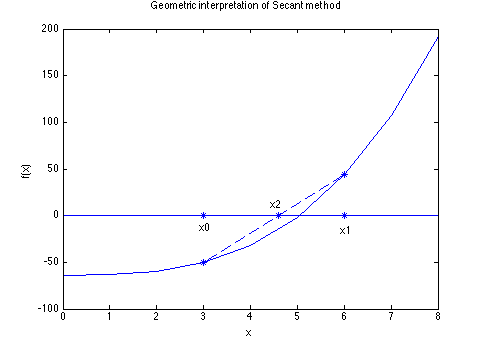
\includegraphics[scale=0.75]{secant}
  \caption{Geometric interpetation of the Secant method for
    root finding.}
  \label{fig:newton}
\end{figure}


\noindent
{\bf MATLAB Code for figure } \\ 
\begin{verbatim} 
x = 0:8;
fx = 0.5 * x.^3 -64;
% Plot the function 
plot(x,fx);
hold on;

x0 = 3;
fx0 = 0.5 * x0.^3-64;
% Plot zero axis 
plot(x, zeros(size(x)));
% plot x0 and f(x2) points
plot(x0,0,'*');
plot(x0,fx0, '*');

% plot x1 and f(x1) points
x1 = 6;
fx1 = 0.5 * x1.^3-64;
plot(x1,0,'*');
plot(x1,fx1, '*');

% plot secant line 
plot([x0,x1],[fx0,fx1],'--');
x2 = x1 - fx1 *(x0-x1)/(fx0-fx1);
plot(x2,0, '*');
hold off;
\end{verbatim} 

\subsection{Example of Secant Method} 

Estimate the root of $f(x) = e^{-x} -x$ employing initial guesses of
$x_{-1} = 0$ and $x_0 = 1$. The iterative equation can be applied to compute: 

\begin{table}[h]
\begin{tabular}{c|c|c} 
$i$ & $x_i$ & $\varepsilon_t(\%)$ \\ 
\hline 
$-1$ & $0$ & $100$ \\
$0$ & $1$ & $76$ \\ 
$1$ & $0.61270$ & $8.03$ \\
$2$ & $0.56384$ & $0.58$ \\ 
$3$ & $0.56717$ & $0.0048$ \\  
\hline
\end{tabular} 
\end{table} 
\noindent 
Notice that the approach converges on the true root faster than 
{\it Bisection} but slower than {\it Newton}.  

\section{Order of convergence of Secant and Bisection} 

The order of convergence of the Secant method derives from the following limit, 
\begin{equation} 
\lim_{i \rightarrow \infty} \left| \frac{E_{i+1}}{E_iE_{i-1}}\right| = \left| \frac{f''(x_t)}{2f'(x_t)} \right|
\end{equation} 
\noindent 
This gives a relationship {\bf between 3 successive errors}. 
However, this does indicate the {\bf order} $\alpha$ of the Secant method, which requires that the errors of 2 successive approximations be related by 
\begin{equation} 
\lim_{i \rightarrow \infty} \frac{|E_{i+1}|}{|E_i|^{\alpha}} = \lambda, \;\;\; \mbox{for some constant } \lambda 
\end{equation} 



It can be shown in fact that, 
\begin{equation} 
\lim_{i \rightarrow \infty} \left| \frac{E_{i+1}}{E_iE_{i-1}}\right| = \lim_{i \rightarrow \infty} \frac{|E_{i+1}|}{|E_i|^{\alpha}} = \left| \frac{f''(x_t)}{2f'(x_t)} \right|
\end{equation}
where 
\[
\alpha = 1 + \frac{1}{\alpha} \implies \alpha^2 - \alpha -1 = 0 \implies \alpha = \frac{1+\sqrt{5}}{2} \approx 1.618 
\]
\noindent 
which is the {\bf order of the Secant method}. 

\noindent 
{\bf Note:} this value $\alpha$ is known as the ``golden ratio'', and occurs in many places in nature as well as many diverse applications. 


An alternate definition of {\bf linear convergence} (similar to the definition given in class except that it does not involve a limit) is: 
\[
|E_i| \leq c|E_{i-1}| \mbox{ or } |x_t - x_i| \leq c |x_t - x_{i-1}|
\]
\noindent 
for some constant $c$ such that $0 < c < 1$. 

Applying this inequality recursively gives 
\[
|x_t - x_i| \leq c^{i} |x_t-x_0|
\]
\noindent 
From page 2 of Handout Number 8, for the Bisection method we had: 
\[
|x_t - x_i| \leq \left( \frac{1}{2}\right)^i \Delta x^0,\mbox{where } \Delta x^{0} = x_u - x_l 
\]
\noindent 
and $[x_l, x_u]$ is the initial interval. This implies linear convergence with the above definition, and $c=\frac{1}{2}$. 
 
\section{Multiple Roots and the Multiplicity of a Zero} 

If Newton's method converges to a zero $x_t$ of $f(x)$, a necessary
condition for quadratic convergence is that $f'(x_t) \neq 0$ . We now
relate this condition on the derivative of $f(x)$ to the multiplicity
of the zero $x_t$.
\vspace{1cm} 

\noindent 
\begin{theorem} (not in textbook)

If $x_t$ is a zero of any analytic function $f(x)$, then there exists a
positive integer $m$ and a function $q(x)$ such that : 

\[
f(x)=(x - x_t)^mq(x),\;\;\mbox{where } \;\; \lim_{x \rightarrow x_t} q(x) \neq 0
\] 

\end{theorem}

(In particular, if $q(x_t)$ is defined, note that $q(x_t ) \neq 0$.) The
value $m$ is called the {\bf multiplicity} of the zero $x_t$. If $m=1$, then 
$x_t$ is called a {\bf simple zero} of $f(x)$. 
\\
{\bf Example 1} Consider 
\[ 
f(x) = x^4 = 9.5 x^3 + 18 x^2 - 56x - 160 = (x+4)^3(x-2.5) 
\]
\noindent 
The zero at $x_t = -4$ has $m=3$ (here $q(x)=x-2.5$ and $q(-4) \neq 0$). \\ 
\noindent 
The zero at $x =2.5$ has $m=1$ (here $q(x)=(x+4)^3$ and $q(2.5) \neq 0$). \\ 

\noindent 
{\bf Example 2}  Consider 
\[
f(x) = e^x - x - 1
\]
\noindent 
Since $f(0)=0$, $x_t =0$ is a zero of $f(x)$. This zero has
multiplicity m=2 since $f(x) = (x-0)^2q(x)$ with $q(x) = \frac{e^x - x
  -1}{x^2}$.

\medskip 
\noindent 
Using l'Hospital's rule we have: 
\[
\lim_{x \rightarrow 0} q(x) = \lim_{x \rightarrow 0} \frac{f(x)}{g(x)} = \lim_{x \rightarrow 0} \frac{f'(x)}{g'(x)} = \lim_{x \rightarrow 0} \frac{e^x -1}{2x} = \lim_{x \rightarrow 0} \frac{e^x}{2} = 0.5 
\]
\noindent 

\begin{theorem} (not in textbook)

Suppose that $f(x)$ and $f'(x)$ are continuous on some interval $[a, b]$, 
and that $x_t \in (a,b)$ and $f(x_t)=0$. Then $x_t$ is a simple zero of $f(x)$ 
if and only if $f'(x_t) \neq 0$. 
\end{theorem}
\noindent 

\begin{proof}

$\Rightarrow$ Suppose first that $x_t$ is a simple zero of $f(x)$. Then 
\[
   f(x) = (x - x_t) q(x), \mbox{where } \lim_{x \rightarrow x_t} q(x) \neq 0
\] 
\noindent 
Therefore, 
\[ 
f'(x) = q(x) + (x - x_t) q'(x) 
\]
\noindent 
and thus 
\[
f'(x_t) = q(x_t) \neq 0
\]

\noindent
$\Leftarrow$ For the converse, suppose that $f'(x_t) \neq 0$. Then by Taylor's Theorem expansion about $a = x_t$, 
\[ 
f(x) = f(x_t) + (x-x_t) f'(\xi)= (x - x_t) f'(\xi) \mbox{ since } f(x_t) = 0
\]
\noindent 
for some value $\xi$ between $x$ and $x_t$. Thus $q(x) = f'(\xi)$ and 
$\lim_{x \rightarrow x_t} q(x) = \lim_{x \rightarrow x_t} f'(\xi) = f'(x_t) \neq 0$. Hence $x_t$ is a simple zero (that is, the multiplicity is $m=1$). 

\end{proof}

\noindent 
The following result follows directly from the above Theorem and our 
previous result about the quadratic convergence of Newton's method.
 
\noindent 
{\bf Corrolary} If Newton’s method converges to a simple zero $x_t$ of $f(x)$, 
then the order of convergence is $2$. 

In order to determine whether or not Newton’s method converges
quadratically to a zero $x_t$ of $f(x)$, you only need to know whether
the multiplicity of $x_t$ is $1$ or is $\geq 2$. The following result
is more general than the above Theorem, and enables you determine the
exact multiplicity of a zero.

\noindent 
\begin{theorem}

Suppose that $f(x)$ and its first $m$ derivatives are continuous on some
interval $[a,b]$ that contains a zero $x_t$ of $f(x)$. Then the
multiplicity of $x_t$ is $m$ if and only if $f(x_t)= f'(x_t) = f''(x_t) = \dots =
f^{(m-1)}(x_t)=0$ but $f^{(m)}(x_t) \neq 0$.
\end{theorem} 

\noindent 
{\bf Example} \\
Consider 
\[ 
f(x) = e^{x} - x - 1
\]

Since $f(0)=0$, $x_t =0$ is a zero of $f(x)$ with multiplicity $m \geq 1.$ \\ 
Since $f'(x) = e^x - 1$ and $f'(0) = 0$, $x_t = 0$ is a zero of $f(x)$ with multiplicity $m \geq 2$. \\
Since $f''(x) = e^{x}$ and $f''(0) \neq 0$, $x_t = 0$ is a zero of $f(x)$ with multiplicity $m=2$. 
\\ 

\newpage
\noindent 
{\bf Significance of multiplicity concerning root-finding algorithms} 

\begin{itemize} 
\item Bracketing methods, such as the Bisection method, cannot be used to compute zeros of {\bf even} multiplicity. 

\item Newton's method and the Secant method both converge only linearly (order of convergence is $\alpha = 1$) if the multiplicity $m$ is $\geq 2$. 

\item A quadratically convergent algorithm for computing a zero $x_t$ of any (unknown) multiplicity of a function $f(x)$ is obtained by applying Newton’s method to the new function. 

\[
u(x) = \frac{f(x)}{f'(x)} 
\] 
\noindent 
rather than to $f(x)$. This is true since if $f(x) = (x-x_t)^m q(x)$ and $m \geq 2$, then 
\[
u(x) = \frac{f(x)}{f'(x)} = \frac{(x - x_t) q(x) }{ m q(x) + (x - x_t) q'(x)}
\] 
\noindent 
has a simple zero $(m=1)$ at $x_t$. By evaluating $u'(x)$, this new algorithm can be written as: 
\[
x_{i+1} = x_i - \frac{u(x_i)}{u'(x_i)} = x_i - \frac{f(x_i)f'(x_i)}{[f'(x_i)]^2 - f(x_i)f''(x_i)}
\]

\end{itemize} 

{\bf Example 5:} Let $f(x)=(x-3)(x-1)^2=x^3-5x^2+7x-3$. Let $x_0 = 0$ and solve with Newton's method and the modified Newton's method. Compare. Do it again for $x_0 = 4$.

In MATLAB,

\begin{verbatim}
>> Newton(0,1e-8,30,@Ex5,@Ex5Prime)
 iteration approximation 
      0 0.0000000000000000 
      1 0.4285714285714286 
      2 0.6857142857142857 
      3 0.8328654004954585 
      4 0.9133298932566344 
      5 0.9557832929657391 
      6 0.9776551012729385 
      7 0.9887661675236611 
      8 0.9943674406865725 
      9 0.9971797713100611 
     10 0.9985888935423050 
     11 0.9992941981316302 
     12 0.9996470368288750 
     13 0.9998235028456799 
     14 0.9999117475293338 
     15 0.9999558727910671 
     16 0.9999779361539637 
     17 0.9999889680091290 
     18 0.9999944840012569 
     19 0.9999972419768860 
     20 0.9999986210059997 
     21 0.9999993105703031 
     22 0.9999996551849977 
     23 0.9999998274423416 
     24 0.9999999123701399 
     25 0.9999999554463016 
     26 0.9999999753813109 
     27 0.9999999844006620 

ans =

    1.0000

>> NewtonMod(0,1e-8,30,@Ex5,@Ex5Prime,@Ex5PrimePrime)
 iteration approximation 
      0 0.0000000000000000 
      1 1.1052631578947369 
      2 1.0030816640986033 
      3 1.0000023814938155 
      4 1.0000000000373122 
      5 1.0000000000746248 

ans =

    1.0000

>> Newton(4,1e-8,30,@Ex5,@Ex5Prime)
 iteration approximation 
      0 4.0000000000000000 
      1 3.3999999999999999 
      2 3.0999999999999996 
      3 3.0086956521739134 
      4 3.0000746407911918 
      5 3.0000000055706231 
      6 3.0000000000000000 

ans =

     3

>> NewtonMod(4,1e-8,30,'Ex5','Ex5Prime','Ex5PrimePrime')
 iteration approximation 
      0 4.0000000000000000 
      1 2.6363636363636367 
      2 2.8202247191011240 
      3 2.9617282104948424 
      4 2.9984787191881508 
      5 2.9999976821826633 
      6 2.9999999999946287 
      7 2.9999999999999996 

ans =

    3.0000
\end{verbatim}



\bibliographystyle{IEEEbib} 
\bibliography{csc349a} 

\end{document} 














